% Created 2024-12-30 Mon 17:39
% Intended LaTeX compiler: pdflatex
\documentclass[11pt,oneside]{memoir}
\makeatletter

\usepackage{answerkey-env}

\ifanswerkey
  \usepackage[forcolorpaper, answerkey]{eqexam}
  \usepackage{vinaya-class-questions}
\else
  \usepackage[forcolorpaper, nosolutions]{eqexam}
  \usepackage[nosolutions]{vinaya-class-questions}
\fi

\proofingsymbolColor{linkred}
\fillinColor{linkred}

\def\maketitle{}

\maxtocdepth{subsection}

\newenvironment{twocols}{%
  \raggedright%
  \setlength{\parindent}{0pt}%
  \setlength{\parskip}{8pt}%
  \fontsize{11}{17}\selectfont%
  \begin{multicols}{2}%
}{%
  \end{multicols}%
}

\newenvironment{widecols}{%
  \hspace*{-0.05\linewidth}\begin{minipage}{1.1\linewidth}%
  \raggedright%
  \setlength{\parindent}{0pt}%
  \setlength{\parskip}{8pt}%
  \fontsize{11}{17}\selectfont%
  \begin{multicols}{2}%
}{%
  \end{multicols}%
  \end{minipage}%
}

\newlength\@tmp@width
\newlength\@tmp@height

\renewcommand*{\printchaptertitleHook}{%
  \AddToShipoutPictureBG*{%
    \put(\LenToUnit{\paperwidth-25mm-\spinemargin},\LenToUnit{\paperheight-95mm}){%
      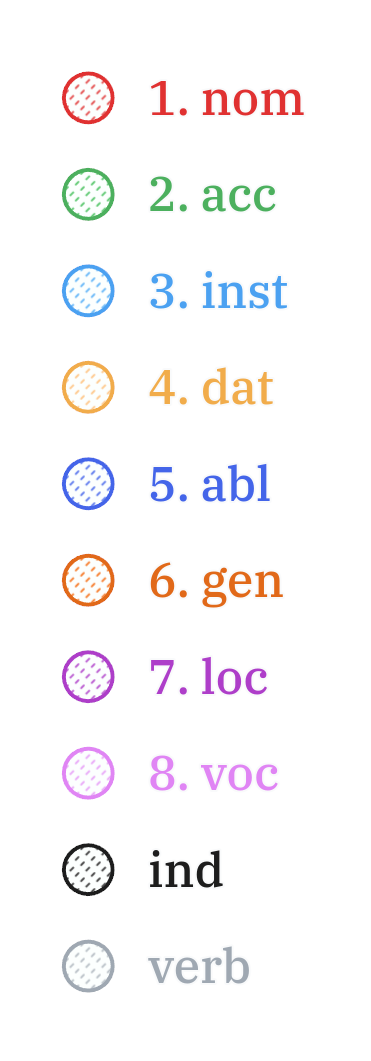
\includegraphics[width=25mm]{./images/cases-legend-white-large.png}%
    }%
  }%
}

\newcommand*\sentenceDiaMsg{\textbf{Exercise:} Draw a sentence analysis diagram below and indicate declensions.}

\newcommand*\sentenceDiaSolution[2][0.4]{%
  \ifanswerkey%
    \hspace*{-\spinemargin}%
    \begin{minipage}{\paperwidth}%
      \centering%
      \includegraphics[scale=#1]{#2}%
    \end{minipage}%
  \else%
    \settototalheight{\@tmp@height}{\includegraphics[scale=#1]{#2}}%
    \begin{minipage}[\@tmp@height]{\linewidth}%
      \sentenceDiaMsg%
    \end{minipage}%
  \fi%
}

\usepackage{cwpuzzle}

\renewcommand\PuzzleCluePre{%
  \begin{minipage}[t]{0.75\linewidth}%
}

\renewcommand\PuzzleClueFont{\fontsize{11}{17}\selectfont}

% \def\PuzzleThickline{\linethickness{2pt}}

\makeatother

\maxtocdepth{section}
\date{\today}
\title{Pāli Readings (Next)}
\hypersetup{
 pdfauthor={The Bhikkhu Saṅgha},
 pdftitle={Pāli Readings (Next)},
 pdfkeywords={},
 pdfsubject={},
 pdfcreator={Emacs 29.4 (Org mode 9.6.15)}, 
 pdflang={En_Gb}}
\begin{document}

\maketitle
\makeatletter

\newlength{\colOne}\setlength{\colOne}{0.35\linewidth}
\newlength{\colTwo}\setlength{\colTwo}{0.6\linewidth}

\renewenvironment{quote}%
{\list{}{%
    \doubleLineSize
    \listparindent 0pt
    \itemindent    0pt
    \leftmargin    3em
    \rightmargin   3em
    \parsep        0pt
    \topsep        8pt
    \partopsep     0pt}%
\item[] \raggedright}%
{\endlist}

\renewcommand*\sentenceDiaSolution[2][0.4]{%
  \ifanswerkey%
    \hspace*{-\spinemargin}%
    \begin{minipage}{\paperwidth}%
      \centering%
      \includegraphics[scale=#1]{#2}%
    \end{minipage}%
  \fi%
}

\makeatother

\mainmatter

\chapter{2024-12-27}
\label{sec:orgf6b07ff}
\section{Ratana sutta: khīṇaṁ purāṇaṁ\ldots{}}
\label{sec:org0156a39}

\begin{quote}
Khīṇaṁ purāṇaṁ navaṁ natthi sambhavaṁ,

Viratta- cittāyatike bhavasmiṁ;

Te khīṇa- bījā avirūḷhi- chandā,

Nibbanti dhīrā yathā- yaṁ padīpo;

Idampi saṅghe ratanaṁ paṇītaṁ,

Etena saccena suvatthi hotu.
\end{quote}

\begin{longtable}{L{\colOne} L{\colTwo}}
khīyati & is destroyed; is exhausted\\[0pt]
khīṇa (pp. of khīyati) & consumed; destroyed\\[0pt]
khaya (m. from khīyati) & wearing away; destruction\\[0pt]
purāṇa (adj.) & previous; old; ancient\\[0pt]
nava (adj.) & new; fresh\\[0pt]
sambhavati & comes to be; happens; occurs\\[0pt]
sambhava (m. from sambhavati) & birth; origin; source (of)\\[0pt]
rajjati & finds pleasure (in); is enamoured (with)\\[0pt]
virajjati & becomes detached (from); loses interest (in)\\[0pt]
viratta (pp. of virajjati) & detached (from); without desire (for); lost interest (in)\\[0pt]
āyati (f.) & future; upcoming\\[0pt]
āyatika (adj. from āyati) & upcoming; future\\[0pt]
bīja (nt.) & seed; germ\\[0pt]
virūḷhi (f.) & growth; increase\\[0pt]
chanda (m.) & (1) interest; desire; wish (2) consent; agreement\\[0pt]
nibbāti & is extinguished; goes out; lit. blows away\\[0pt]
dhīra (adj.) & (1) stable; constant; reliable; firm (2) wise; intelligent\\[0pt]
padīpa (m.) & lamp; light; lighting\\[0pt]
\end{longtable}

(tesaṁ,) purāṇaṁ kammaṁ khīṇaṁ hoti

navaṁ sambhavaṁ natthi

kammaṁ: nt. nom/acc. sg.

kammaṁ khettaṁ, viññāṇaṁ bījaṁ, taṇhā sneho (AN 3.76)
\end{document}
